% Created 2026-04-22 Wed 22:24
% Intended LaTeX compiler: lualatex
\DocumentMetadata{lang = en, pdfversion = 2.0, pdfstandard = ua-2, pdfstandard = a-4, testphase = {phase-III, title, table, math, firstaid}}
\documentclass[11pt]{article}
\usepackage{amsmath}
\usepackage{fontspec}
\usepackage{graphicx}
\usepackage{longtable}
\usepackage{wrapfig}
\usepackage{rotating}
\usepackage[normalem]{ulem}
\usepackage{capt-of}
\usepackage{hyperref}
\usepackage[margin=1in]{geometry}
\usepackage{fontspec}
\usepackage{verbatim, multicol, tabularx,}
\usepackage{amsmath, amsthm, amssymb, stmaryrd, latexsym, bm, listings, qtree}
\usepackage{framed}
\usepackage{xcolor,colortbl}
\usepackage{media9}
\usepackage[export]{adjustbox}
\usepackage{algorithm}
\usepackage[noend]{algpseudocode}
\usepackage{tikz,pgfplots}
\usetikzlibrary{shapes.geometric}
\let\oldquote=\quote
\let\endoldquote=\endquote
\colorlet{shadecolor}{cyan!15}
\renewenvironment{quote}{\begin{shaded*}\begin{oldquote}}{\end{oldquote}\end{shaded*}}
% From https://tex.stackexchange.com/questions/7032/good-way-to-make-textcircled-numbers
\newcommand*\circled[1]{\tikz[baseline=(char.base)]{\node[shape=circle,draw,inner sep=2pt] (char) {#1};}}
\DeclareMathOperator*{\argmin}{arg\!min}
\DeclareMathOperator*{\argmax}{arg\!max}
\lstset{frame=tb, aboveskip=1mm, belowskip=0mm, showstringspaces=false, columns=flexible, basicstyle={\scriptsize\ttfamily}, numbers=left, frame=single, breaklines=true, breakatwhitespace=true}
\hypersetup{colorlinks=true,urlcolor=blue}
\usepackage{polyglossia}
\setdefaultlanguage[variant=US]{english}
\author{Christopher Simpkins}
\date{Kennesaw State University}
\title{Artificial Intelligence\\\medskip
\large Value Alignment}
\hypersetup{
 pdfauthor={Christopher Simpkins},
 pdftitle={Artificial Intelligence},
 pdfkeywords={},
 pdfsubject={Artificial Intelligence Value Alignment},
 pdfcreator={Emacs 30.2 (Org mode 9.7.11)}, 
 pdflang={English}}
\begin{document}

\maketitle
\section{What is a value?}
\label{sec:orgfed653e}

In ethical theory, how "good" something is.

\begin{itemize}
\item Value of a goal
\item Value of an action
\end{itemize}

Values lead to hierarchies.

\begin{itemize}
\item Cookies vs. health
\end{itemize}

\url{https://plato.stanford.edu/entries/value-theory/}
\section{Value Alignment in AI}
\label{sec:orgc49df39}

Today we'll focus on two broad areas of value alignment in AI:

\begin{itemize}
\item \textbf{supervised statistical machine learning}, in which harmful biases in arise in pattern learning, and
\item \textbf{autonomous agents}, which we want to have human-aligned goals and \textbf{behavior}.
\end{itemize}
\section{Good Goals, Harmful Outcomes}
\label{sec:orgb2f288b}

Amazon's Sexist Hiring Tool

\begin{itemize}
\item Resume evaluator trained on 10 yers of hiring data
\item Most software engineers are male
\item Tool learned from data to prefere males
\end{itemize}

\url{https://www.technologyreview.com/2018/10/10/139858/amazon-ditched-ai-recruitment-software-because-it-was-biased-against-women/}
\section{The Genie Problem}
\label{sec:orgaea3301}






\includegraphics[alt={diverse nazis},height=3.0in]{diverse-nazis.png}






\begin{itemize}
\item Value: diversity
\item Result: inacurate and offensive images
\end{itemize}
\section{AI Snake Oil}
\label{sec:org1b69a9c}





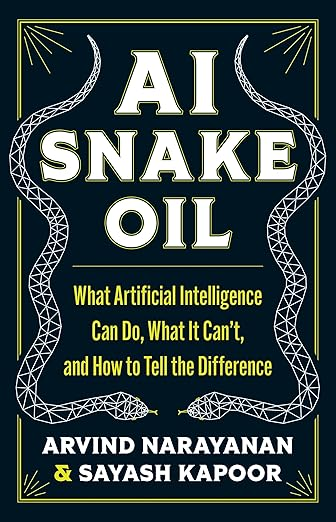
\includegraphics[alt={ai snake oil book},height=3.0in]{ai-snake-oil-book.jpg}






\begin{itemize}
\item AI, like other products, tends to be oversold
\item As AI engineers we need to be aware of AI's limitations
\end{itemize}

\begin{quote}
It all comes down to honesty.
\end{quote}
\section{At least some AI companies are honest aobut their goals.}
\label{sec:org9a6fabe}



\includegraphics[alt={palantir saruman},height=3.0in]{palantir-saruman.png}
\section{Value Alignment as a Focus of AI Research}
\label{sec:org0c1499c}





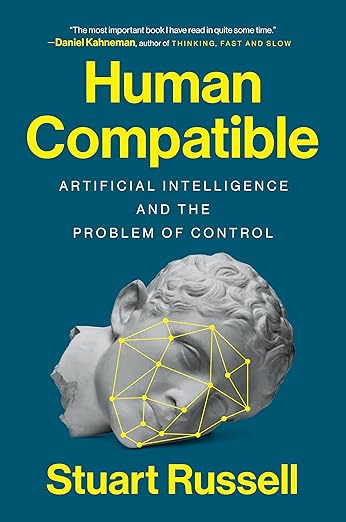
\includegraphics[alt={human compatible book},height=3.0in]{human-compatible-book.jpg}







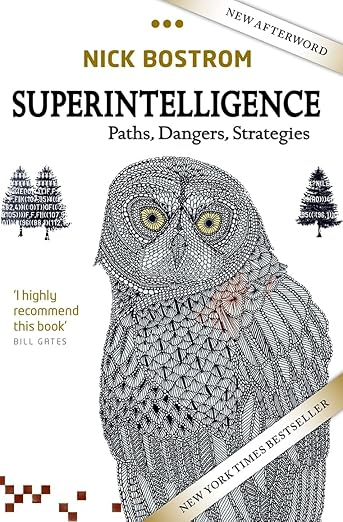
\includegraphics[alt={superintelligence book},height=3.0in]{superintelligence-book.jpg}
\section{Value Alignment in Autonomous Agents}
\label{sec:orgc7a1e73}






\textbf{Bad advice can be dangerous.}\\
\vspace{.1in}
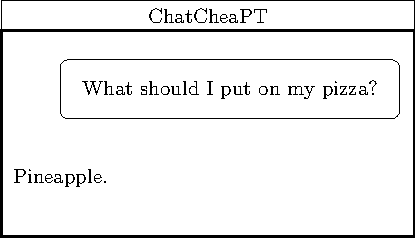
\includegraphics[alt={chatcheapt pineapple pizza advice},height=1.0in]{chatcheapt-pineapple-pizza-advice.pdf}





\rule{0.5pt}{.35\textheight}




\textbf{Bad action is worse.}\\
\vspace{.1in}
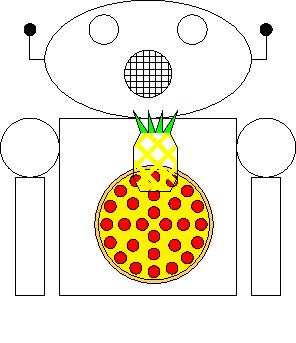
\includegraphics[alt={robot serving pineapple pizza},height=1.2in]{robot-serving-pineapple-pizza.pdf}














\includegraphics[alt={christopher simpkins headshot 600px},height=1.0in]{christopher-simpkins-headshot-600px.jpg}


\includegraphics[alt={chris.simpkins.phd qr},height=1.0in]{chris.simpkins.phd-qr.png}

\textbf{Christopher Simpkins}\\
\small{Kennesaw State University}\\
\small\{\url{https://chris.simpkins.phd/}\}




\rule{0.5pt}{.4\textheight}



\textbf{General Interests}

\begin{itemize}
\item Multiagent systems
\item Reinforcement learning
\item Deep learning
\item Causality
\item \ldots{}
\end{itemize}

\textbf{Current thrust}: MARL approaches to value alignment
\section{Value Alignment as a Theory of Mind Problem}
\label{sec:org378209c}






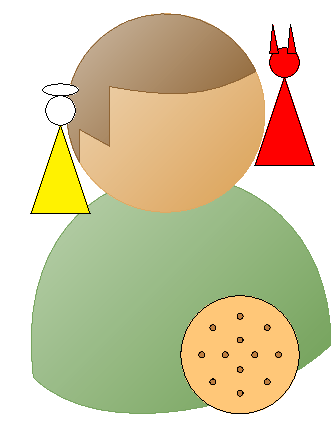
\includegraphics[alt={angel demon},height=1.4in]{angel-demon.pdf}





\rule{0.5pt}{.4\textheight}






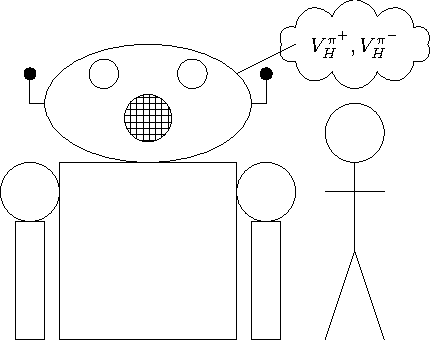
\includegraphics[alt={robot mtom},height=1.4in]{robot-mtom.pdf}












\textbf{Goal: learn values from behavior.}

\begin{itemize}
\item Not just "don't run over pedestrians" but "don't harm humans."
\item Start with action restrictions
\item Learning approach

\begin{itemize}
\item Don't replace the Genie Problem with the knowledge acquisition bottleneck/bitter lesson.
\end{itemize}
\end{itemize}



\rule{0.5pt}{.4\textheight}




\textbf{Advances needed:}

\begin{itemize}
\item Machine theory of mind
\item Imitation/apprenticeship learning
\item Offline reinforcement learning
\item World models -- causality
\end{itemize}

\textbf{Impacts:}

\begin{itemize}
\item Autonomous multi-agent systems
\item Human-AI teaming
\item Safe autonomy
\end{itemize}






This is my note.

\begin{itemize}
\item It can contain Markdown
\item like this list
\end{itemize}
\section{Choosing Actions}
\label{sec:org3516612}

Elements of outcomes can be more or less desirable -- more or less \textbf{useful} -- to a given agent.

\begin{itemize}
\item Utility is the quality of being useful.
\item That "usefulness" may simply be pleasure, or even altruism.
\end{itemize}

Utility theory associates a utility value with each possible outcome, which induces a preference ordering over outcomes.

\begin{quote}
An agent is rational if and only if it chooses the action that yields the highest expected utility, averaged over all the possible outcomes of the action.
\end{quote}

Each action, \(a\), leads to a probability distribution over outcomes, or "result states":

$$
\sum_{s \in S} Pr(s) = 1
$$

And each outcome state has a utility.  A rational decision-theoretic agent chooses the action that maximize expected utility, that is:

$$
\argmax_{a} \sum_{s \in S} Pr(s) U(s)
$$
\section{Values, Utilities, Rewards, Goals}
\label{sec:orga249bb9}

\begin{itemize}
\item Values: general concept
\item Utility: quality of being useful
\item Reward: feedback from the enbvironment
\item Goal: state of the environment satisfying set of conditions
\end{itemize}

Coconut cupcakes.
\section{Reinforcement Learning in a Few Slides}
\label{sec:orgc58afb3}

An intelligent agent learns how to behave from experience interacting with the world.

\begin{itemize}
\item We represent subsets of the world as \textbf{environments} comprised of \textbf{states}..
\item An \textbf{agent} takes an \textbf{action} that causes a transition to a new state.
\item The agent receives a scalar feedback signal, called a \textbf{reward}, from the environment after the transition to a new state.
\item The agent maximizes the long-term expected value of cumulative reward.
\end{itemize}

Reinforcement learning directly addresses the intelligent agent problem.  Its central hypothesis is:

\begin{quote}
All of what we mean by goals and purposes can be well thought of as the maximization of the expected value of the cumulative sum of a received scalar signal (called reward).[\textsuperscript{SuttonBarto2018}]
\end{quote}

{[}\textsuperscript{SuttonBarto2018}]: ttp://incompleteideas.net/book/the-book-2nd.html
\section{Markov Process}
\label{sec:org9a338d9}

A markov process models the world as a set of states and associated transition probability distributions, calles a \textbf{transition function}, that models how the world moves from one state to the next.

\[
Pr(s_{t+1} | s_t)
\]

is the probability that the state at time \(t+1\) is \(s_{t+1}\), given that the previous state is \(s_t\).  The fact that the transition probability depends only on the previous state and not the history of all previous states is called the \textbf{Markov assumption}.


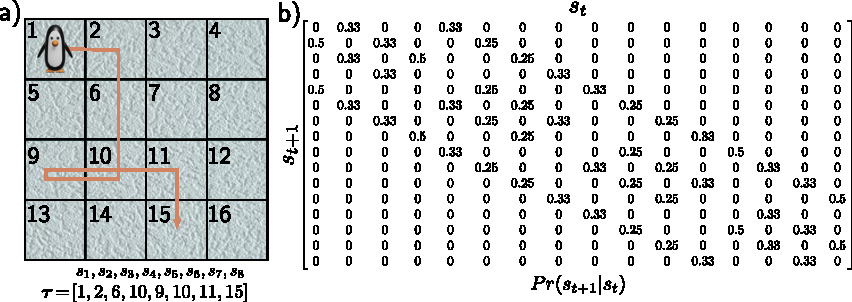
\includegraphics[alt={../../deep learning/slides/ReinforceMDP},height=1.6in]{../../deep-learning/slides/ReinforceMDP.pdf}



A sequense of states from a Markov process is called a \textbf{trajectory}: \(\tau = (s_1, S_2, ...)\).
\section{Markov Reward Process}
\label{sec:org692a10e}

A \textbf{Markov reward process} adds a reward distribution \(Pr(r_{t+1} | s_t)\) (note that this implicitly accompanies a state transition).  Now a trajectory includes the rewards, \(\tau = (s_1, r_2, s_2, r_3...)\), and the sum of cumulative discounted future rewards, the \textbf{return}, is:

\[
G_t = \sum_{k = 0}^\infty \gamma^k r_{t+k+1}
\]

\(\gamma\) is the \textbf{discount factor} which says how much we discount future rewards.  With \(\gamma < 0\) it decays to zero.


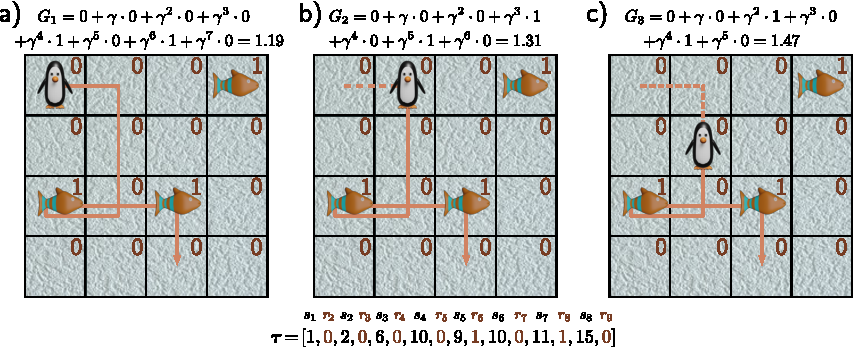
\includegraphics[alt={../../deep learning/slides/ReinforceMDP2},height=1.6in]{../../deep-learning/slides/ReinforceMDP2.pdf}
\section{Markov Decision Process (MDPs)}
\label{sec:orgad4d04f}

A \textbf{Markov decision process} (MDP) adds a set of \textbf{actions} at each time step.  Now:

\begin{itemize}
\item transition probabilities are \(Pr(s_{t+1} | s_t, a_t)\).  Sometimes written as \(T(s, a, s')\) -- a \textbf{transition model} that returns the probability that taking action \(a\) in state \(s\) results in state \(s'\).
\item the reward probabilities are \(Pr(r_{t+1} | s_t, a_t)\).  This is sometimes written as \(r(s, a, s')\)
\item a trajectory is \(\tau = (s_1, a_1, r_2, s_2, a_2, r_3...)\)
\end{itemize}


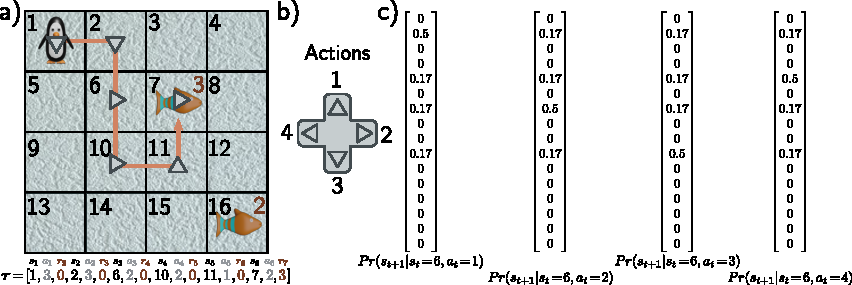
\includegraphics[alt={../../deep learning/slides/ReinforceMDP3},height=2.0in]{../../deep-learning/slides/ReinforceMDP3.pdf}
\section{Policy}
\label{sec:orgc90d480}

The goal of a reinforcement learning algorithm is to learn a \textbf{policy}: a deterministic or stochastic function mapping states to actions.

\begin{itemize}
\item Stationary: \(\pi(a | s)\)
\item Non-stationary: \(\pi(a_t | s_t)\)
\end{itemize}


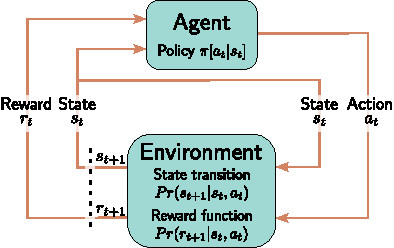
\includegraphics[alt={../../deep learning/slides/ReinforceMDPLoop},width=0.75\linewidth]{../../deep-learning/slides/ReinforceMDPLoop.pdf}
\section{State and Action Values}
\label{sec:org8f18eaf}

\begin{itemize}
\item State value function: \(v(s_t | \pi) = \mathbb{E} [G_t | s_t, \pi]\)
\item Action value function: \(q(s_t, a_t | \pi) = \mathbb{E} [G_t | s_t, a_t, \pi]\)
\end{itemize}


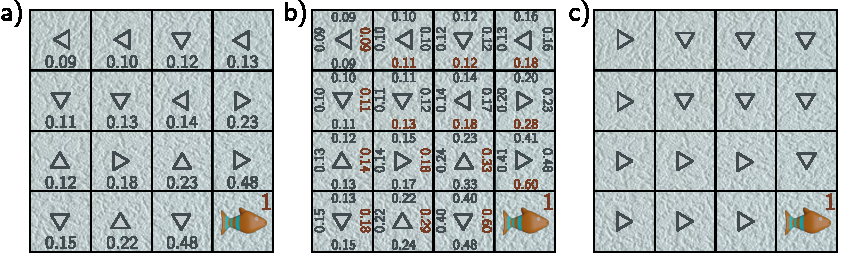
\includegraphics[alt={../../deep learning/slides/ReinforceValueOfAction},width=0.75\linewidth]{../../deep-learning/slides/ReinforceValueOfAction.pdf}
\section{Optimal Policy}
\label{sec:org4539b1c}

An optimal policy maximizes the expected return.  Any MDP has a deterministic stationary optimal policy, i.e., it maximizes the value of every state.  Given this policy:

\[
v^*(s_t ) = \max_{\pi} \big( \mathbb{E} [G_t | s_t, \pi] \big)
\]

The optimal action value function is then:

\[
q^*(s_t, a_t ) = \max_{\pi} \big( \mathbb{E} [G_t | s_t, a_t \pi] \big)
\]

If we know \(q^*\) we can use it to derive \(\pi^*\):

\[
\pi^*(a_t | s_t ) \leftarrow \argmax_{a_t} \big( q^*(s_t, a_t ) \big)
\]

We'll see this idea when we solve MDPs using dynamic programming.
\section{Bellman Equations}
\label{sec:org3e7f46f}

If we substitute the action value function into the state value function we get:

\[
v(s_t ) = \sum_{a_t} \pi(a_t | s_t) \big( r(s_t, a_t) + \gamma \sum_{s_{t+1}} Pr(s_{t+1} | s_t, a_t) v(s_{t+1})  \big)
\]

If we substitute the state value function into the action value function we get:

\[
q(s_t, a_t) = r(s_t, a_t) + \gamma \sum_{s_{t+1}} Pr(s_{t+1} | s_t, a_t) \Huge( \sum_{a_{t+1}} \pi(a_{t+1} | s_{t+1}) q(s_{t+1}, a_{t+1})  \Huge)
\]

These two relations are called the \textbf{Bellman equations}.  They say that state and action values mult be self-consistent, so when we update the estimated value of a state or actoin, we have to update all the others that depend on the updated value.
\section{Tabular RL}
\label{sec:orga6de144}

In classical tabular RL, we represent the policy function as a table.

\begin{itemize}
\item Model-based: use the MDP to solve for the best policy.

\begin{itemize}
\item Policy iteration
\item Value iteration
\end{itemize}

\item Model-free: estimate from observed trajectories

Q-Learning

\begin{equation}
Q(s, a) \gets Q(s, a) + \alpha [R(s) + \gamma \max_{a'} Q(s', a') - Q(s, a)]
\end{equation}

SARSA

\begin{equation}
Q(s, a) \leftarrow Q(s, a) + \alpha [R(s) + \gamma Q(s', a') - Q(s, a))]
\end{equation}
\end{itemize}

In modern RL we approximate the various functions -- \(V(s)\), \(Q(s, a)\), \(\pi(s)\) -- using supervisd machine elarning, most notably deep neural networks ("deep RL").
\section{Machine Theory of Mind}
\label{sec:orge8f917b}

An agent develops a model of how another agent thinks.  For RL, can model other agent's:

\begin{itemize}
\item Value function
\item Reward function
\item Policy
\end{itemize}
\end{document}
